\section{Messungen}
\subsection{Verwendete Geräte}

	\begin{itemize}
		\item Oszilloskop
		\begin{itemize}
			\item Tektronix TDS 3014C Digital Phosphor Oszilloscope
		\end{itemize}
		
		\item Puls-Generator
		\begin{itemize}
			\item Hewlett Packard 33120A 15MHz Function/Arbitary Waveform Generator
		\end{itemize}
		
		\item Kabel
		\begin{itemize}
			\item 1m BNC Kabel
		\end{itemize}
		
		\item Audio Analyzer
		\begin{itemize}
			\item Rhode \& Schwarz UPV Audio Analyzer DC...250kHz
		\end{itemize}
		
		\item Messobjekt
		\begin{itemize}
			\item Universalfilter
		\end{itemize}
		
		\item BNC Stecker - T-Stücke
	\end{itemize}


\newpage

\subsection{Messung von Amplituden- und Phasengang}
\noindent In diesem Versuch geht es darum, die Amplituden und Phasengänge der Butterworth-, Tschebyscheff- und Bessel-Tiefpässe und die Amplitudengänge der Butterworth-, Tschebyscheff- und Bessel-Hochpässe sowie des Bandpasses und der Bandsperre mittels dem Audio-Analyzer UVP zu messen. Die folgende Tabelle zeigt unsere gemessenen Grenzfrequenzen der Tiefpässe/Hochpässe. Die Graphen sind im Anhang zu finden.

	\begin{table}[h]
		\centering
		\begin{tabular}{c|c|c|c|}
					& Butterworth	& Tschebyscheff	& Bessel  \\
			\hline
			Tiefpass& $1.538kHz$	& $1.557kHz$	& $1.551kHz$  \\
			Hochpass& $1.596kHz$    & $1.592kHz$	& $1.610kHz$  \\   
		\end{tabular}
		\caption{Gemessenen Grenzfrequenzen der verschieden Tiefpässe/Hochpässe}
		\label{tab:grenzfrequnzen_hp_tp}
	\end{table}
	
\noindent Anschließend ging es darum, die Phasengänge der oben genannten Filtertypen für den Tiefpass zu messen. Die Frequenzen bei einer Phasenverschiebung von $-60^\circ$ und $-120^\circ$ wurden bestimmt und in die folgende Tabelle eingetragen. Auch diese Graphen sind im Anhang zu finden.

\begin{table}[h]
	\centering
		\begin{tabular}{c|c|c|c|}
						& Butterworth	& Tschebyscheff	& Bessel  \\
			\hline		
		    $-60^\circ $& $1.046kHz$    & $898.250kHz$	& $1.229kHz$  \\
			$-120^\circ$& $2.381kHz$    & $1.400kHz$	& $3.225kHz$  \\   
	\end{tabular}
	\caption{Frequenzen bei einer Phasenverschiebung von $-60^\circ$ und $-120^\circ$ }
	\label{tab:phasenverschiebung_hp_tp}
\end{table}
	
\noindent Schließlich wurden die Mittenfrequenz und Sperrfrequenz des Bandpasses sowie der Bandsperre gemessen. Ergebnisse sind der folgenden Tabelle zu entnehmen. Für die Graphen siehe Anhang.

\begin{table}[h]
	\centering
	\begin{tabular}{c|c|c|}
					& Mittenfrequenz & Sperrfrequenz  \\
		\hline
		Bandpass	& $1.556kHz$     & -         \\
		Bandsperre	& -              & $1.568kHz$  \\   
	\end{tabular}
	\caption{Mittenfrequenz und Sperrfrequenz, Bandpass und Bandsperre}
	\label{tab:grenzfrequnzen_bs_bp}
\end{table}

\newpage

\subsection{Sprungantworten der Tiefpässe}
\noindent In diesem Versuch geht darum, die Anstiegszeit, Überschwingen und die Einstiegszeit der drei Tiefpässe nach Butterworth, Tschebyscheff und Bessel aus der Sprungantwort zu bestimmen. Die Filter wird mit einem Rechtecksignal ($500mV_pp$ und $250mv$ Offset und variabler Frequenz) angesteuert. Eingangs- und Ausgangssignal werden in einem gemeinsamen Oszillogramm dargestellt. Der Messaufbau ist in der nachfolgenden Abbildung zu sehen.

\begin{figure}[h]
\centering
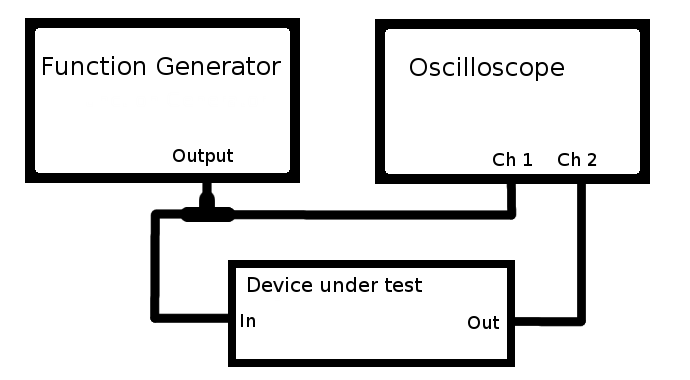
\includegraphics[width=0.7\linewidth]{Bilder/Messaufbau_Oszi}
\caption{Messaufbau zum Messen der Sprungantwort}
\label{fig:Messaufbau_Oszi}
\end{figure}


\begin{figure}[h]
\centering
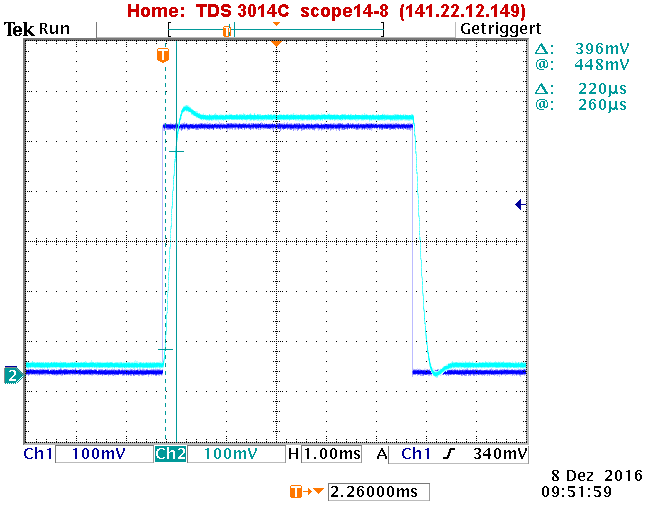
\includegraphics[width=0.7\linewidth]{Bilder/ImLabor/Sprungantwort_5_8_Butter_Anstiegszeit}
\caption{Sprungantwort Butterworth-Tiefpass}
\label{fig:Sprungantwort_5_8_Butter_Anstiegszeit}
\end{figure}

\begin{figure}[h]
\centering
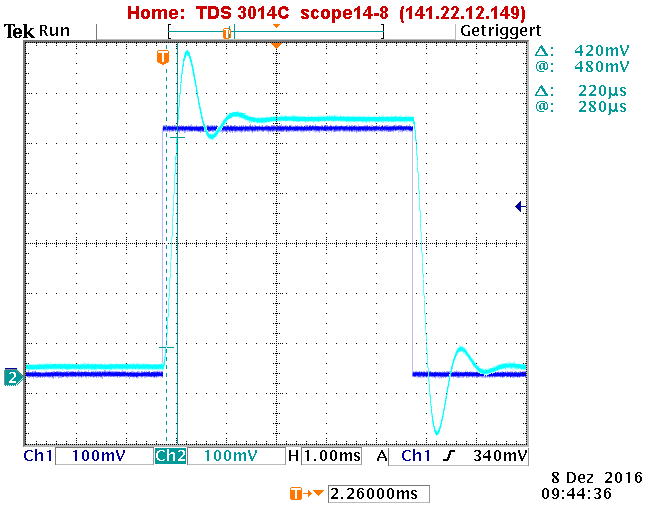
\includegraphics[width=0.7\linewidth]{Bilder/ImLabor/Sprungantwort_5_3_Tscheby_Anstiegszeit}
\caption{Sprungantwort Tschebyscheff-Tiefpass}
\label{fig:Sprungantwort_5_3_Tscheby_Anstiegszeit}
\end{figure}

\begin{figure}[h]
\centering
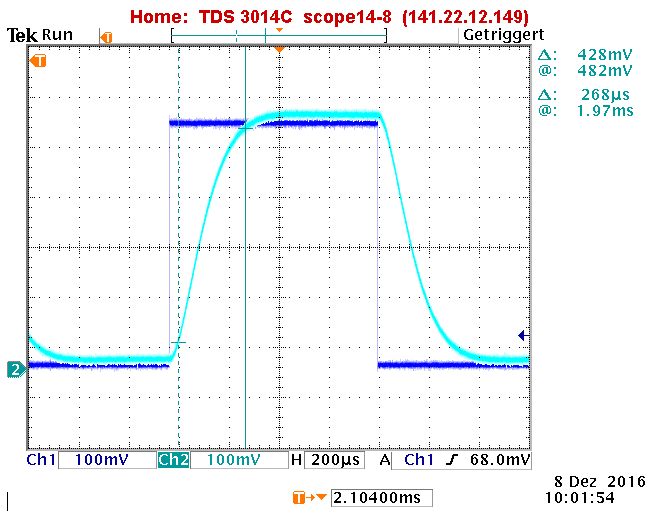
\includegraphics[width=0.7\linewidth]{Bilder/ImLabor/Sprungantwort_5_1_Bessel_Anstiegszeit}
\caption{Sprungantwort Bessel-Tiefpass}
\label{fig:Sprungantwort_5_1_Bessel_Anstiegszeit}
\end{figure}

\newpage